\documentclass[12pt,a4paper]{article}
\usepackage[utf8]{inputenc}

\usepackage{multicol}
\usepackage{graphicx}
\usepackage{fancyhdr}
\usepackage{times}
\usepackage{titlesec}
\usepackage{multirow}
\usepackage{lettrine}
\usepackage{hyperref}
\usepackage{subfig}
\usepackage[demo]{graphicx}
\usepackage[top=2cm, bottom=1.5cm, left=2cm, right=2cm]{geometry}
\usepackage[figurename=Fig.,tablename=TAULA]{caption}


\author{\LARGE\sffamily Marc Maldonado Lorca}
\title{\Huge{\sffamily Data Science: Estimación del peso de un cerdo \\
Informe De Seguimiento 1}}

\date{}

\newcommand\blfootnote[1]{%
  \begingroup
  \renewcommand\thefootnote{}\footnote{#1}%
  \addtocounter{footnote}{-1}%
  \endgroup
}
\renewcommand{\contentsname}{whatever}
\renewcommand{\refname}{Referencias}
%
%\large\bfseries\sffamily
\titleformat{\section}
{\large\sffamily\scshape\bfseries}
{\textbf{\thesection}}{1em}{}

\begin{document}

\fancyhead[LO]{\scriptsize Marc Maldonado Lorca: Estimación del peso de un cerdo}
\fancyhead[RO]{\thepage}
\fancyhead[LE]{\thepage}
\fancyhead[RE]{\scriptsize EE/UAB TFG INFORMÀTICA: Estimación del peso de un cerdo}

\fancyfoot[CO,CE]{}

\fancypagestyle{primerapagina}
{
   \fancyhf{}
   \fancyhead[L]{\scriptsize TFG EN ENGINYERIA INFORMÀTICA, ESCOLA D'ENGINYERIA (EE), UNIVERSITAT AUTÒNOMA DE BARCELONA (UAB)}
   \fancyfoot[C]{\scriptsize ``Noviembre'' de 2021, Escola d'Enginyeria (UAB)}
}

%\lhead{\thepage}
%\chead{}
%\rhead{\tiny EE/UAB TFG INFORMÀTICA: Estimación del peso de un cerdo}
%\lhead{ EE/UAB \thepage}
%\lfoot{}
%\cfoot{\tiny{February 2015, Escola d'Enginyeria (UAB)}}
%\rfoot{}
\renewcommand{\headrulewidth}{0pt}
\renewcommand{\footrulewidth}{0pt}
\pagestyle{fancy}

%\thispagestyle{myheadings}


%\vspace*{-1cm}{\scriptsize TFG EN ENGINYERIA INFORMÀTICA, ESCOLA D'ENGINYERIA (EE), UNIVERSITAT AUTÒNOMA DE BARCELONA (UAB)}

\maketitle

\thispagestyle{primerapagina}
%\twocolumn[\begin{@twocolumnfalse}
%\maketitle
%\begin{abstract}
\begin{center}
\parbox{0.915\textwidth}
{\sffamily

}
\bigskip

{\vrule depth 0pt height 0.5pt width 4cm\hspace{7.5pt}%
\raisebox{-3.5pt}{\fontfamily{pzd}\fontencoding{U}\fontseries{m}\fontshape{n}\fontsize{11}{12}\selectfont\char70}%
\hspace{7.5pt}\vrule depth 0pt height 0.5pt width 4cm\relax}

\end{center}

\bigskip
%\end{abstract}


\section{Contexto y objetivos}

Desde hace unos años el sector agrario evoluciona junto a las nuevas tecnologías emergentes, lo que se conoce como Smart Farming. Este nuevo concepto aprovecha el potencial de las TIC para abaratar tanto los costes de producción como la eficiencia de las granjas. A partir de esta idea se han ideado nuevos modelos de gestión que van desde los invernaderos inteligentes y la gestión de plagas, hasta la implementación de drones agrícolas que utilizando imágenes aéreas permiten un ahorro significativo de tiempo y mano de obra a la hora de la verificación visual de un cultivo. Ademas no solo es aplicable al cultivo sino que existe una interesante aplicación en el ganado. 



Es por eso que el CVC trabajó en un proyecto de Smart Farming relacionado con la automatización de una granja de cerdos, donde uno de los retos pendientes era estimar el peso de los estos con la motivación de conocer su evolución y prepararlos para dar el peso optimo en el matadero y así obtener la máxima rentabilidad posible. A la hora de entregar un cerdo al matadero su valor depende de lo que se aproxime su peso a loas 120kg, este valor del animal disminuye tanto si su peso es inferior o superior al estándar establecido, es por eso que el control de la evolución de estos animales es tan importante para obtener beneficios. 


El concepto consiste en utilizar una cámara 3D para hacer fotos cenitales de los animales y así eliminar el costoso proceso de utilizar una bascula y agilizar el pesaje aumentando de esta manera el numero de cerdos pesados por unidad de tiempo \cite{sistema}.

Este problema ya ha sido planteado por muchas personas, instituciones y empresas, además de haber sido abordado de distintas maneras y con distintos animales. Se han utilizado imágenes 2D donde se segmenta al cerdo utilizando técnicas de morfología, se construye su esqueleto y con las medidas de este utilizando una regresión se obtiene el peso \cite{Area}. En otro estudio utilizando vacas y una reconstrucción 3D similar a nuestros datos y extrayendo diferentes atributos como la altura, la anchura, el área, etc, consiguen estimar mediante regresión el peso de la vaca entre otros factores\cite{3D}.
También existe otra solución utiliza imágenes de profundidad con las cuales utilizando redes neuronales convolucionales consigue estimar tanto el peso como otras variables biométricas del animal \cite{CNN}.
Finalmente otro estudio mediantes nubes de puntos como las que disponemos y analizando la postura de los cerdos, analizando la relación entre volumen y postura del animal consiguen mediante regresión estimar el peso.


Además de todos estos estudios ya existen productos en el mercado variados con diferentes enfoques.
La empresa PLF AGRITECH \cite{PLF} ha puesto en práctica diferentes tecnologías para el desarrollo de los animales en las granjas inteligentes, aportan una solución al problema de la detección de peso además de un alimentador automático inteligente y un control sobre el impacto medioambiental de estas grajas en términos de aire.
FANCOM \cite{fancom} a parte de tener productos enfocados al crecimiento de otros animales como los pollos o productos destinado al cultivo de hongos también aportan una solución al control del peso de los cerdos con su producto EYEGROW \cite{fancomvideo}. Con una cámara de profundidad en el techo ellos son capaces de segmentar los cerdos individualmente y estimar el peso de ellos simultáneamente para después con la ayuda de un software poder analizar la evolución. Para esta tarea es interesarte leer un articulo de SENSORS \cite{deteccion} que bajo el pretexto de la existencia de pocos datasets de cerdos ofrecen un modelo capaz de identificar a estos en fotos cenitales ademas de identificar la posición de sus distintas partes del cuerpo. Una aplicación similar a la anterior es la de GROSTAT \cite{GroStat}.
\begin{figure}[!]
\centering
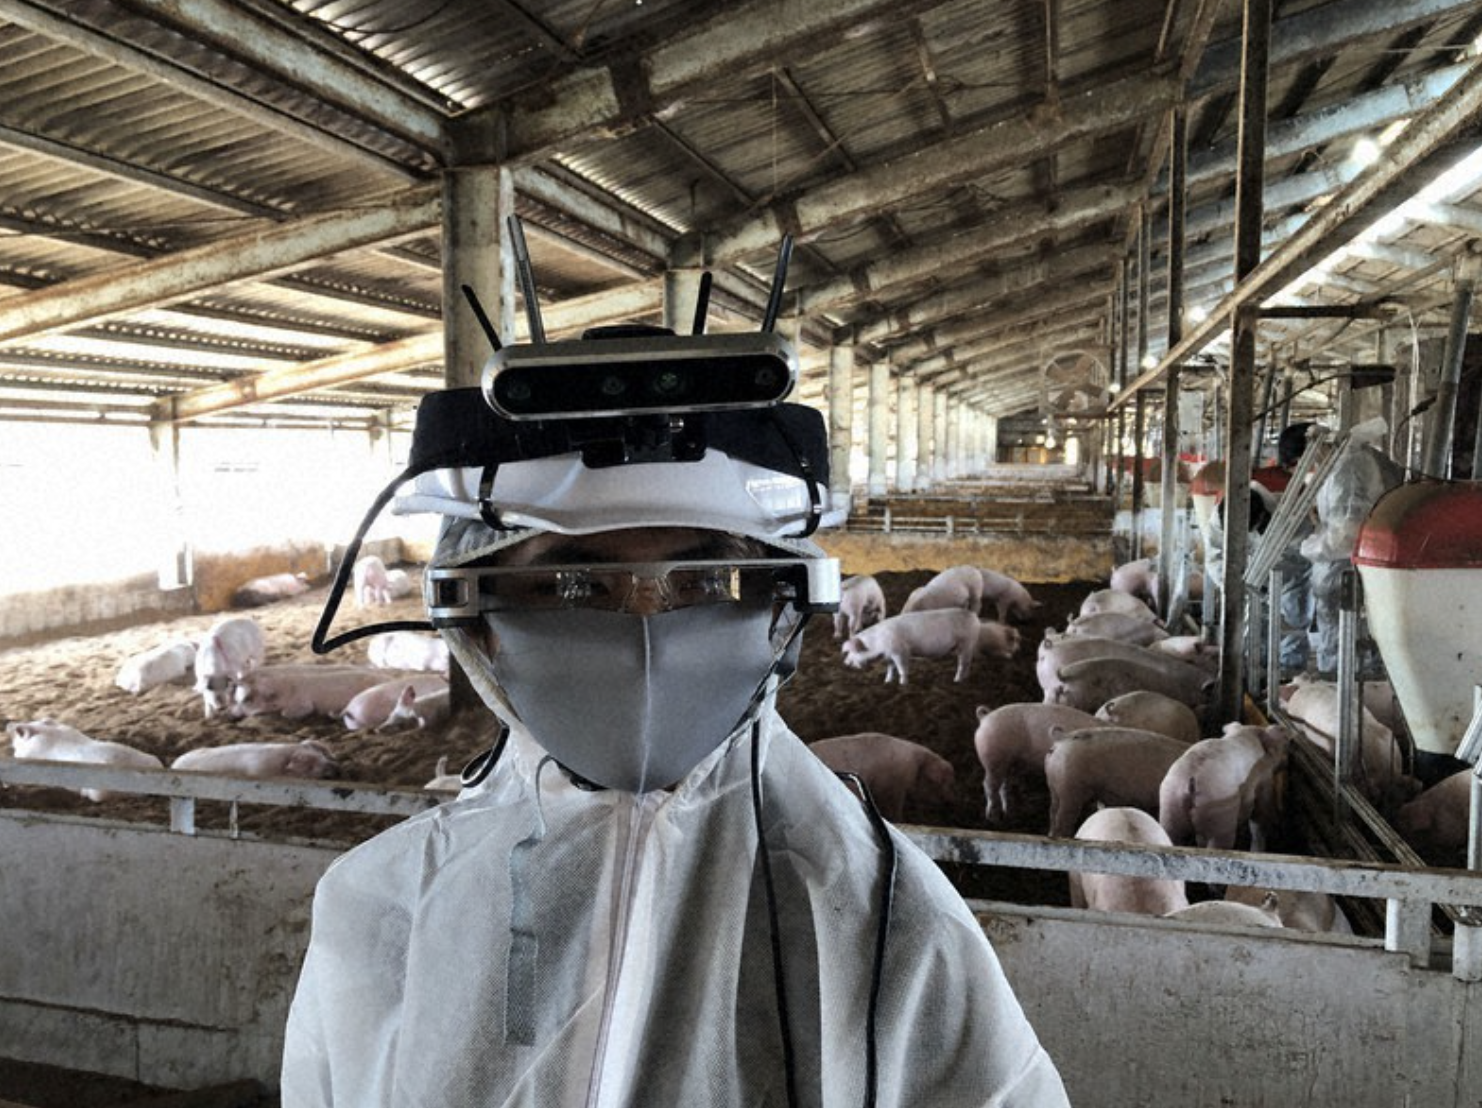
\includegraphics[width=0.3\textwidth]{05-TFG-template-latex/images/gafas.png}
\caption{Gafas de realidad virtual para la estimación de peso}
\label{gafas}
\end{figure}

\begin{figure}[h]
\centering
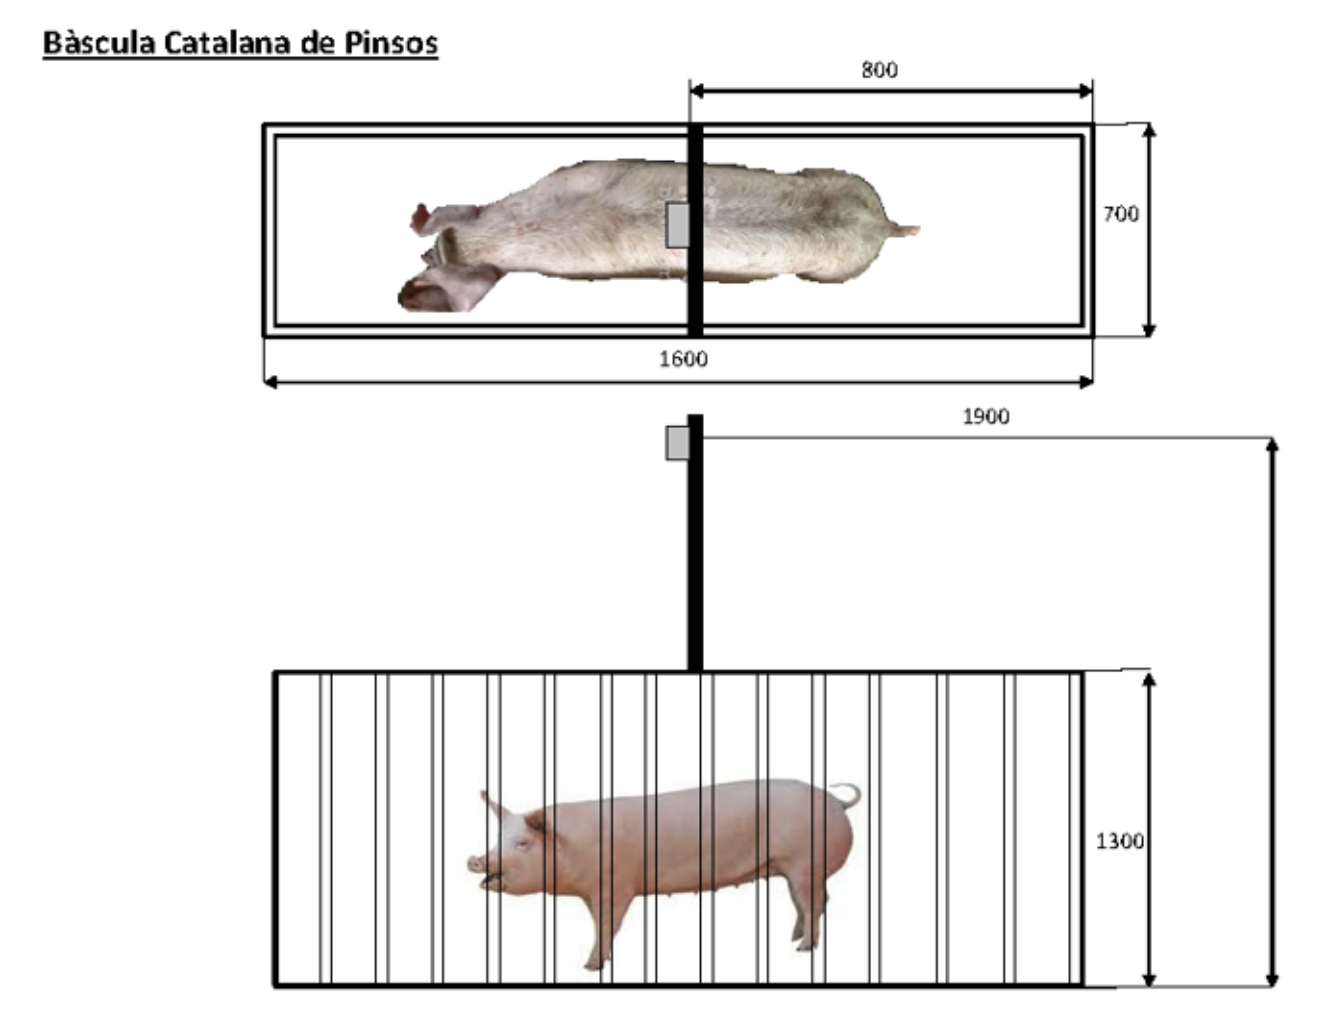
\includegraphics[width=0.4\textwidth]{05-TFG-template-latex/images/montaje.png}
\caption{Báscula con montaje de la camara}
\label{montaje}
\end{figure}

\begin{figure}
\centering
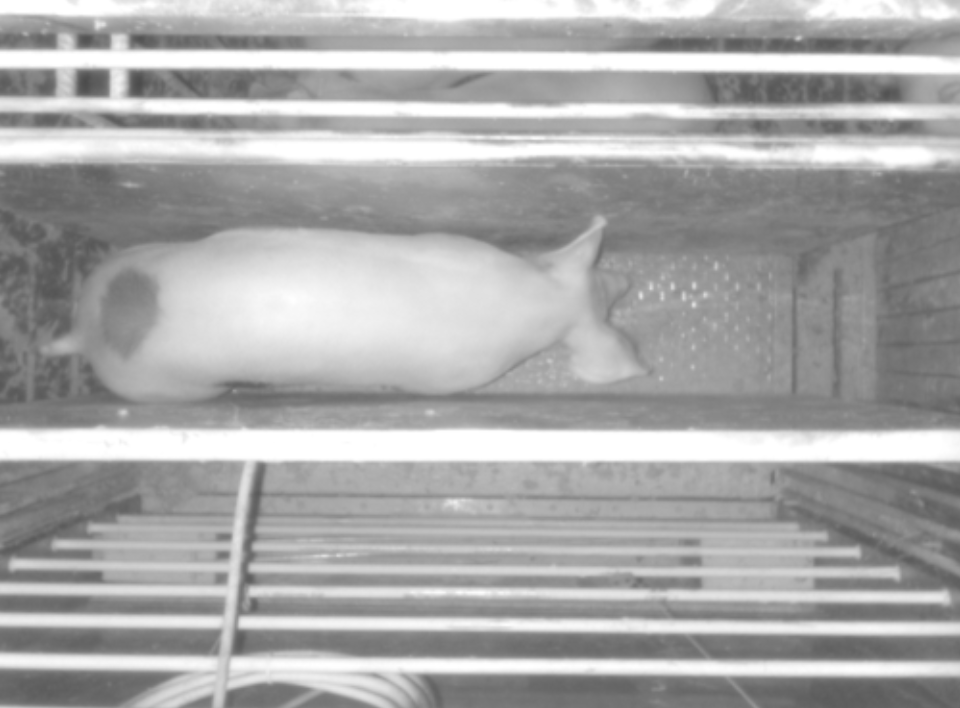
\includegraphics[width=0.3\textwidth]{05-TFG-template-latex/images/foto.png}
\caption{Ejemplo de imagen cenital}
\label{foto}
\end{figure}

Existe un enfoque diferente en cuanto a la manera de utilizar la cámara, mientras empresas como la anterior deciden colocar la cámara en un lugar fijo, otras empresas optan por la manipulación de la cámara de manera manual, de esta manera se facilitaría la selección del cerdo a pesar. Es el caso de H+L \cite{H+L} o PIGGY CHECK \cite{piggycheck} que mediante cámaras 3D incorporadas en dispositivos móviles consiguen estimar los pesos de los cerdos de manera individual. Existe una solución similar desarrollada por Southwest Japan univ. \cite{japon} pero esta vez la cámara está acoplada a unas GOOGLE glasses \cite{google} como se muestra en la \textbf{Fig \ref{gafas}} de manera que tan solo mirando al cerdo tendríamos la información, aunque todavía no se ha lanzado al mercado.
El peso es un buen indicador de la salud del cerdo pero no es suficiente, DEGREE2ACT \cite{degree} ha desarrollado un gadget para smartphone que mediante una cámara de temperatura nos informa de posibles enfermedades del cerdo, lo cual junto a una estimación del peso podría ser una potente herramienta.

Analizando el contexto y la distribución de nuestra la granja y teniendo en cuenta el recorrido que realizaban los cerdos, se instaló en la báscula tradicional la cámara 3D BASTER BLAZE \cite{camara}, la cual se adapta bien por su resistencia, encargada de recoger el modelo 3D de los cerdos, con imágenes como la que se muestra en la \textbf{Fig \ref{foto}}, y su peso real, todo esto con la ayuda de células fotosensibles que controlarían la entrada individual de cada cerdo a la báscula, además de la instalación de un lector RFID y los respectivos PLC y PC, el montaje se muestra en las \textbf{Fig \ref{montaje}} para procesar y almacenar los datos obtenidos en forma de nube de puntos.


El objetivo real del proyecto extraer el potencial del dataset de las nubes de puntos utilizando modelos de machine learning y encontrar la solución más óptima posible al problema de la estimación del peso de un cerdo utilizando una cámara 3D. En un futuro esta solución combinada a distintas ideas podría ser un producto con bastante potencial.







\section{Metodología}

Durante la realización de esta primera parte del proyecto se ha proseguido con el planteamiento del informe inicial siguiendo la planificación de las fechas del TFG además de cada semana hacer reuniones individuales con el tutor para así comentar los avances y poder corregir errores. La metodología decidida en el kick-off del proyecto fue la ágil, concretamente Kanban utilizando el software de JIRA \cite{JIRA} que además proporciona herramientas como el diagrama de Gantt. Por el momento está decisión parece ser adecuada y se amolda perfectamente a la hora de desarrollar el proyecto. Como se explicó en el informe inicial, siguiendo esta hoja de ruta y el método Kanban organizaremos las tareas dentro de cuatro apartados en un tablero:



\begin{itemize}
  \item \textbf{POR HACER: }Aquí se colocarán todas las tareas que todavía no se han empezado a hacer, de aquí solo se podrán mover a la columna EN PROGRESO.
  \item \textbf{EN PROGRESO: }Aquí se colocarán las tareas que se encuentran en desarrollo, solo se podrán mover hacia el estado EN REVISIÓN.
  \item \textbf{EN REVISIÓN: }Esta columna contiene las tareas acabadas pendientes de revisión por el tutor, en el caso de completarse satisfactoriamente se moverán a HECHO, en el caso contrario volverán a EN PROGRESO.
  \item \textbf{HECHO: }Este apartado contendrá las tareas finalizadas.
\end{itemize}




\section{Planificación}

Se planificaron diversas tareas en el primer informe que durante su ejecución han ido cambiando, eliminándose o añadiendo nuevas.

\begin{table}[!]
 \centering
\begin{tabular}{|c|c|c|}
\hline
\textbf{Fase 1}             & \textbf{Fase 2}                  & \textbf{Fase 3}    \\ \hline
Estudio Dataset             & Tratamiento datos de peso        & Informe final      \\
Visualización datos         & Estudio métodos de regresión     & Presentación final \\
Segmentación clásica        & Entrenar GNN peso                &                    \\
Conversión a nube de puntos & Entrenar CNN peso                &                    \\
Detección de  objetos       & Analisis resultados              &                    \\
Segmentación semantica      & Comparativa con otras soluciones &                    \\
Limpieza de máscaras        & Informe de progreso 2            &                    \\
Informe de progreso 1       &                                  &                    \\ \hline
\end{tabular}
\caption{Backlog}
\label{backlog}
\end{table}

\begin{figure}[h]
\centering
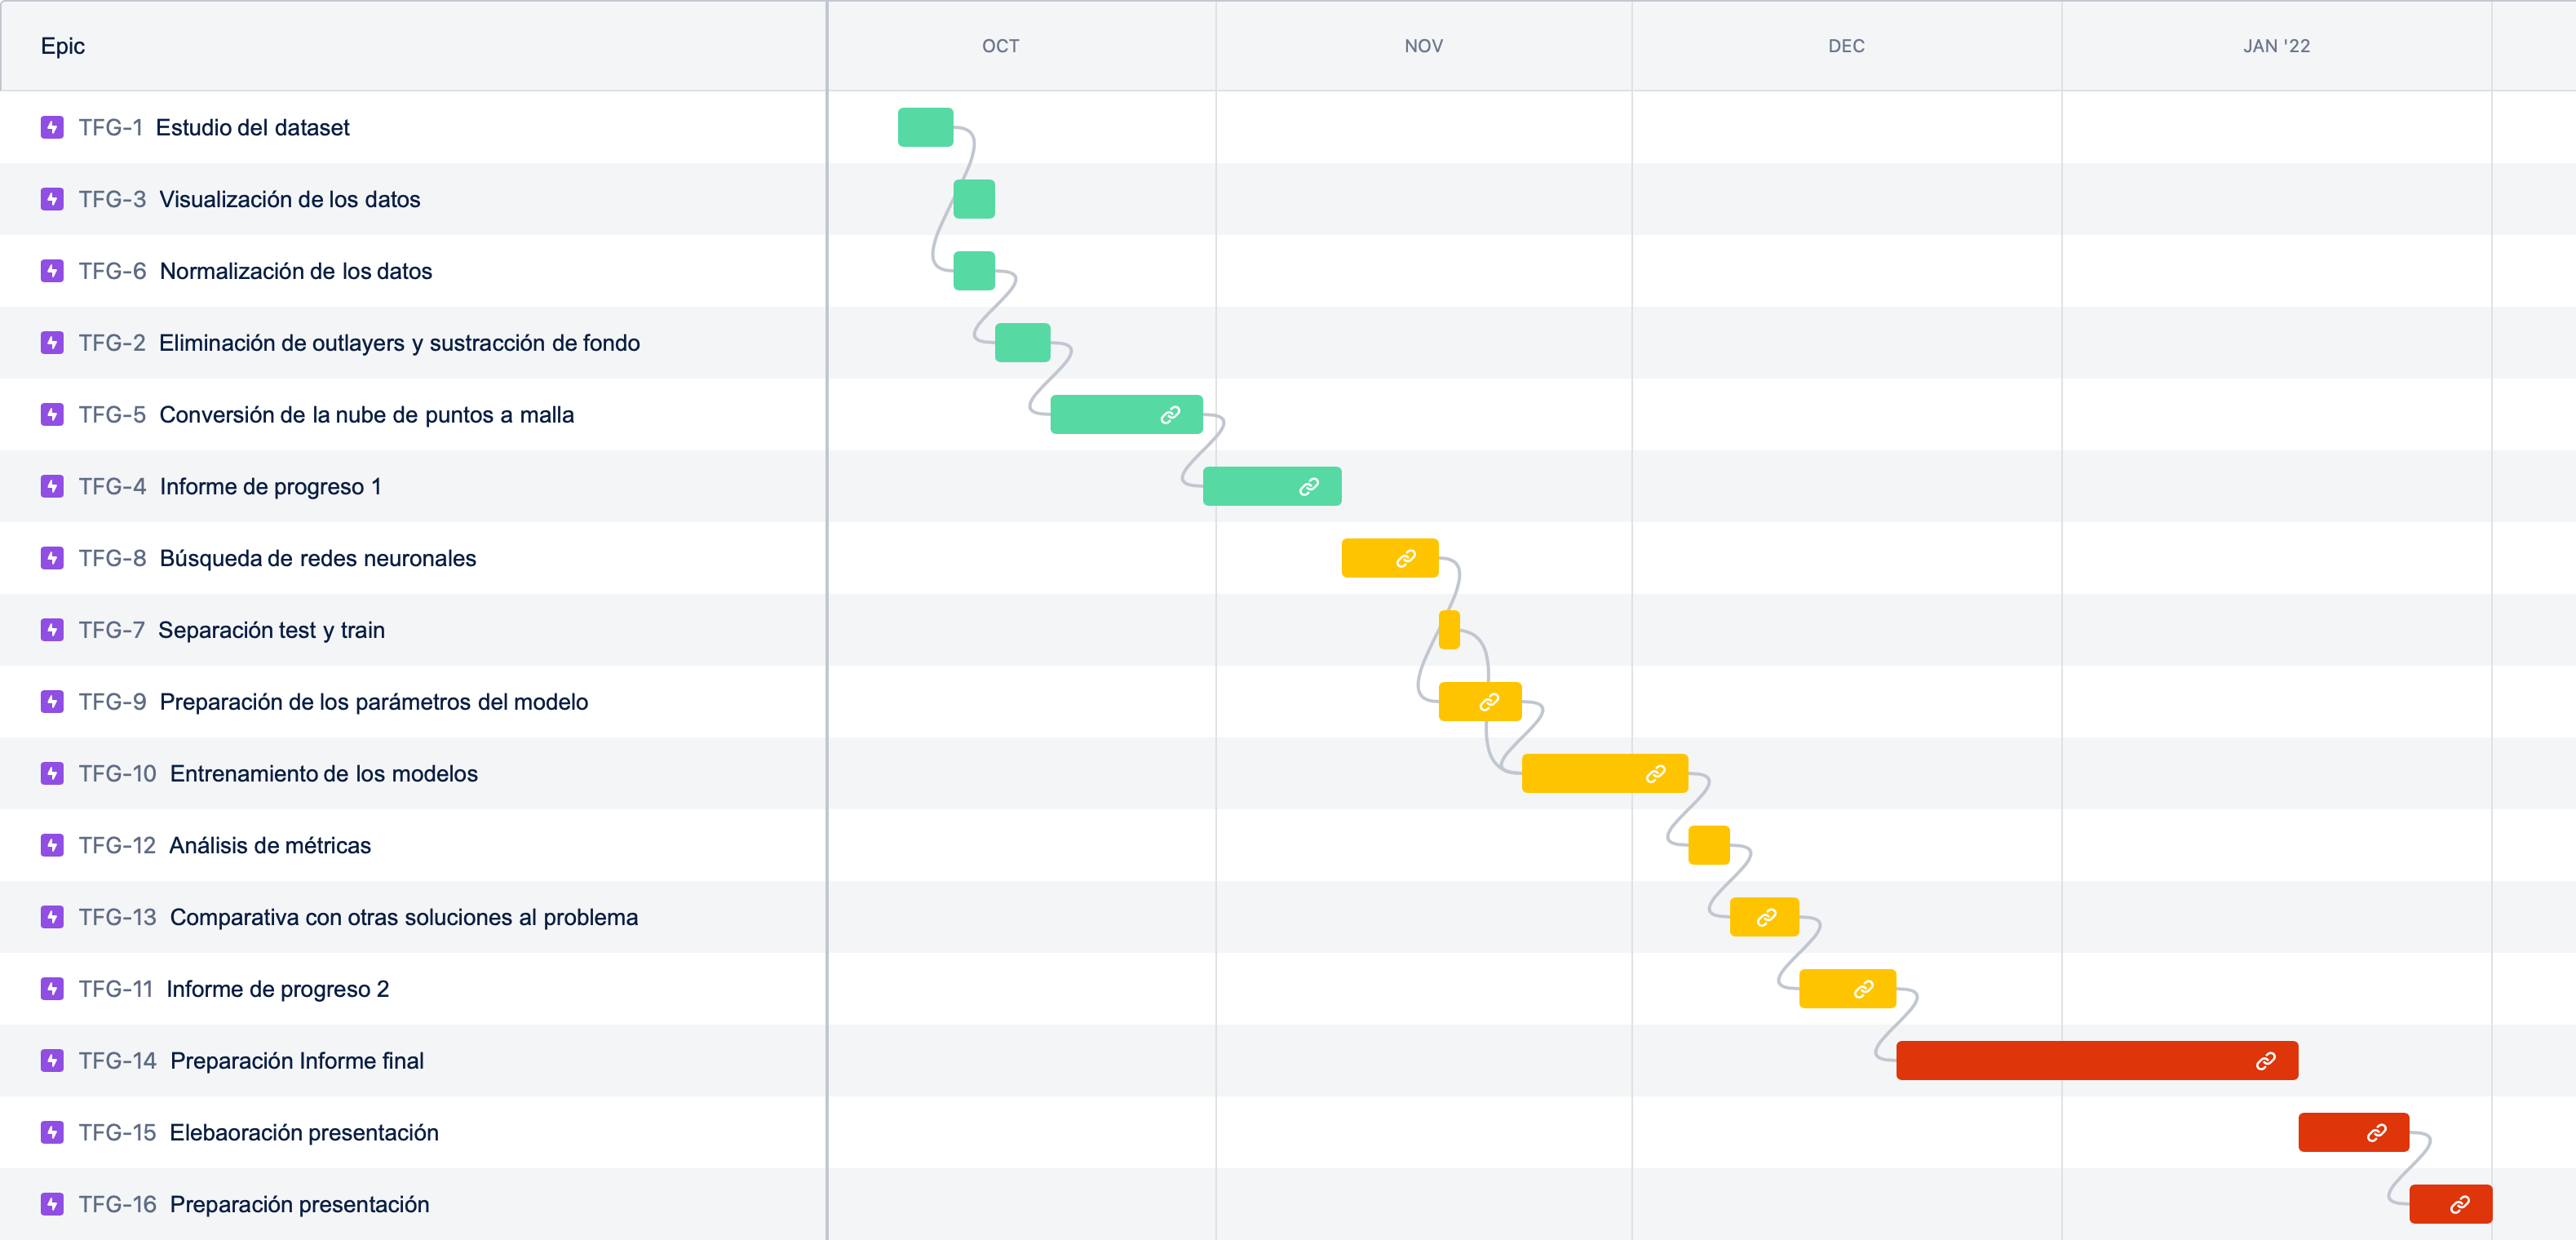
\includegraphics[width=0.8\textwidth]{05-TFG-template-latex/images/gant.png}
\caption{Diagrama de Gantt}
\label{gant}
\end{figure}


En la \textbf{Fig \ref{gant}} y en la \textbf{TAULA \ref{backlog}} se muestran la nueva planificación de tareas que conforman el proyecto repartidas por semanas.

La parte de la segmentación de los cerdos se podría dar por finalizada aunque se trabajará en desarrollar un modelo de segmentación semántica más ligero como MobileNetv2 \cite{mobilenet}, ya que es posible que genere muy buenos resultados.

El siguiente paso es transformar las nubes de puntos en mallas.
Seguidamente, se limpiarán y prepararán los datos de los pesos para entrenar modelos de regresión.
En este punto se tratará de desarrollar dos soluciones distintas, una utilizando las imágenes tridimensionales experimentando con CNN y otra utilizando las mallas generadas para entrenar una GNN. Todo esto previamente habiendo estudiado las distintas arquitecturas.
Se compararán los resultados y se extraerán conclusiones.
Esta idea sobre la planificación puede cambiar al avanzar el proyecto.







\section{Desarrollo}

Están parte del desarrollo se ha focalizado en la segmentación de los cerdos experimentando con diferentes técnicas.

\begin{figure}[ht]%
 \centering
 \subfloat[]{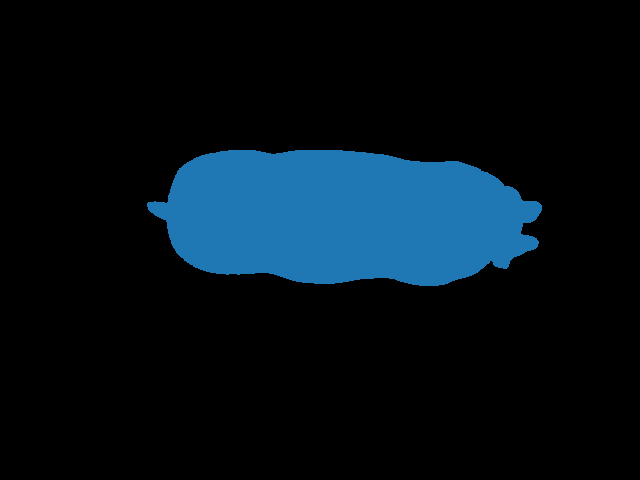
\includegraphics[scale=0.2]{05-TFG-template-latex/images/gt.png}\label{fig:a}}%
 \subfloat[]{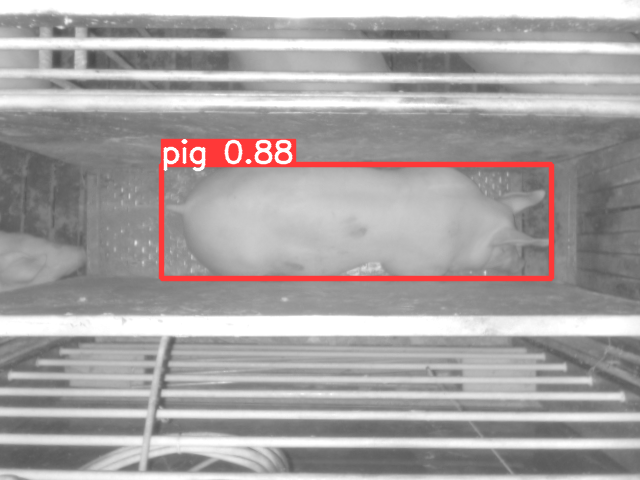
\includegraphics[scale=0.2]{05-TFG-template-latex/images/YOLOBOX.png}\label{fig:b}}\\
 \subfloat[]{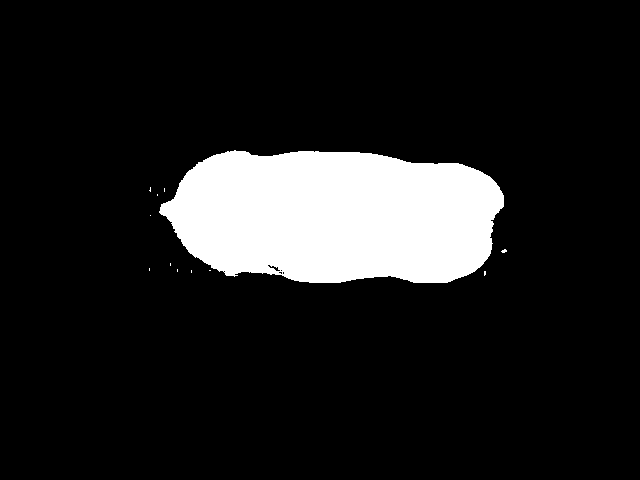
\includegraphics[scale=0.2]{05-TFG-template-latex/images/YOLO.png}\label{fig:c}}%
 \subfloat[]{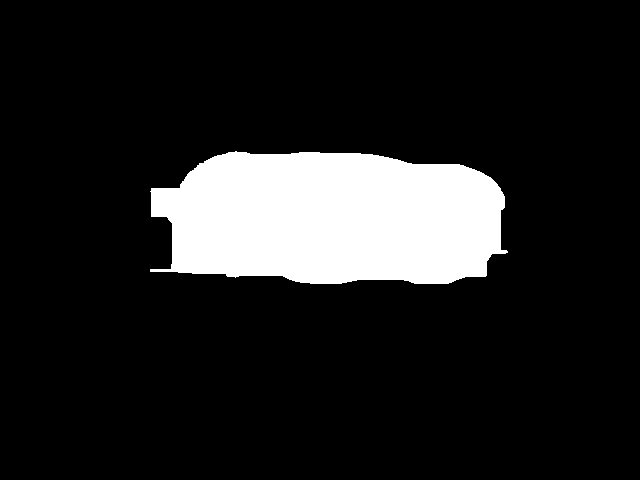
\includegraphics[scale=0.2]{05-TFG-template-latex/images/YOLOrefinado.png}\label{fig:d}}%
 \caption{Proceso de segmentación YOLO}%
 \label{yoloimg}%
\end{figure}


Primero, al no disponer de suficiente cantidad de imágenes ni de una imagen de la báscula vacía se intentó mediante la media de todas las imágenes generar una nueva la cual se usaría como fondo, esto se hizo tanto con las imágenes de la cámara de infrarrojos como con las imágenes de profundidad, estos métodos han sido bautizados como \textbf{Mean} y \textbf{Mean 3D} respectivamente. Una vez con esta nueva imagen generada se realiza una subtracción a cada imagen de cerdos para tratar de eliminar el fondo, antes habiéndole aplicado un suavizado gausiano para tratar de conseguir un resultado más limpio. Seguidamente probando thresholds manuales o utilizando Otsu\cite{Otsu}. Generamos la máscara final. Haciéndolo con las imágenes de infrarrojas genera resultados notablemente mejores que con las imágenes de profundidad.

Seguidamente, se proporcionó una imagen de fondo para hacerle la subtracción, de la misma manera con las dos imágenes, estos métodos son los de \textbf{Difference} y \textbf{Difference3D}. Esta vez en vez de hacer la media de todas las imágenes realizamos la resta directamente con el fondo. De la misma manera se aplica un filtro de suavizado y con thresholds manuales y Otsu se generan las nuevas máscaras. Estas técnicas obtienen un rendimiento similar a las dos técnicas anteriores solo que a la inversa. En cuanto al uso de imágenes infrarrojas, este resultado se debe a que ahora a diferencia del anterior, utilizamos una imagen del fondo, debido a la superficie de la báscula se genera un reflejo de luz de un color similar al lomo del cerdo, así que la mayoría de los cerdos están segmentados por todo su cuerpo menos por la parte que coincide con el reflejo, esto explica la perdida de precisión. La mejora empleando imágenes de profundidad respecto al anterior método usando las mismas se debe a que existe una diferencia en el fondo de la imagen. Aquí es donde nos dimos cuenta de que una de las paredes de la báscula cambiada de posición dependiendo de la fotografía. Esto se debe a que las paredes se ajustan dependiendo del tamaño de los animales para no permitir que entren dos simultáneamente. Aun de esta manera de todas las images disponibles existen un gran número con la pared en la misma posición respecto a demás imágenes con la pared en distinta posición. Al ser la imagen del fondo una representante las imágenes que más se repiten en cuanto a posición de la pared, por eso genera tan buenos resultados.

Aquí es cuando probamos \textbf{Otsu} directamente con la imagen infrarroja, con las imágenes de profundidad queda directamente descartado, ya que segmentaría muchas partes de la báscula que para eliminarlas después utilizando morfología sería una tarea muy difícil. Hacerlo directamente con Otsu funciona bien pero no mejor que \textbf{Difference3D}.

En este punto se puede ver que el verdadero problema se encuentra con el fondo y no con los cerdos así que se busca una solución, la primera es utilizar Canny y Hough\cite{hough} para detectar las líneas de la báscula y así eliminar el problema de las paredes móviles y el fondo. Esta técnica funciona bien con el primer conjunto de imágenes, al tener nuevas se vuelve un reto imposible debido a la variedad de fotos, de este modo, se descarta y se opta por un recorte horizontal de la imagen que elimine fondo, pero no interfiera ni recorte en ningún caso alguna parte del cerdo, seguidamente aplica Otsu sobre el recorte. Hasta el momento esta técnica bautizada como \textbf{Otsu\_crop} se convierte en la mejor técnica para segmentar.

También se experimenta usando Niblack y Sauvola \cite{Niblack}, pero no se obtienen ningún resultado a apreciar.

Viendo el potencial de recortar la imagen se decide generar groundtruths para entrenar un modelo de segmentación semántica, para esto se utiliza la herramienta Hasty.ai \cite{hasty} la cual proporciona diversas herramientas para el etiquetado de imágenes, a nivel semántico, de objeto y de imagen. En este caso se hizo semanticamente, ya que a partir de aquí también podemos generar bounding boxes para la detección de objetos. Esta herramienta permite etiquetar de manera simultánea con demás personas y durante el etiquetado entrena modelos que te ofrecen una posible mascara la cual tú puedes editar. Con este groudtruth se extrajeron las bounding boxes y usando Google Colab se entrenó un modelo \textbf{Yolo}\cite{yolo}, concretamente V5, con el cual se recorta al cerdo y se aplica Otsu sobre la imagen recortada. Genera un resultado similar a Otsu\_crop, pero ligeramente peor en cuanto accuracy, de todas maneras elegimos Yolo porque la diferencia es ínfima y nos asegura que siempre cogemos al cerdo y no otros cerdos que asoman la cabeza por la puerta como se puede ver en alguna imagen. Además, sobre estas máscaras generadas se aplica técnicas de morfología para rellenar huecos dentro de los cerdos generados por las manchas de estos y kernels horizontales para tratar de dilatar horizontalmente la máscara y recuperar puntos pertenecientes al cerdo no segmentados. \cite{yolo} para con su detección tener una imagen recortada del cerdo y aplicar Otsu sobre él. El proceso de segmentación se puede ver en la \textbf{Fig \ref{yoloimg}} siendo \textbf{\subref{fig:a}} el groundtruth, \textbf{\subref{fig:b}} la detección de Yolo, \textbf{\subref{fig:c}} Otsu aplicado sobre la detección de Yolo y \textbf{\subref{fig:d}} aplicando la morfología.

  \begin{table}[!]
\centering
\begin{tabular}{|l|l|}
\hline
Difference   & 0.47 \\ \hline
Difference3D & 0.87 \\ \hline
Mean         & 0.81 \\ \hline
Mean3D       & 0.36 \\ \hline
Otsu         & 0.69 \\ \hline
Otsu\_crop   & 0.97 \\ \hline
Yolo         & 0.97 \\ \hline
\end{tabular}
\caption{Accuracy métodos segmentación}
\label{acc}
\end{table}

\begin{figure}[!]
\centering
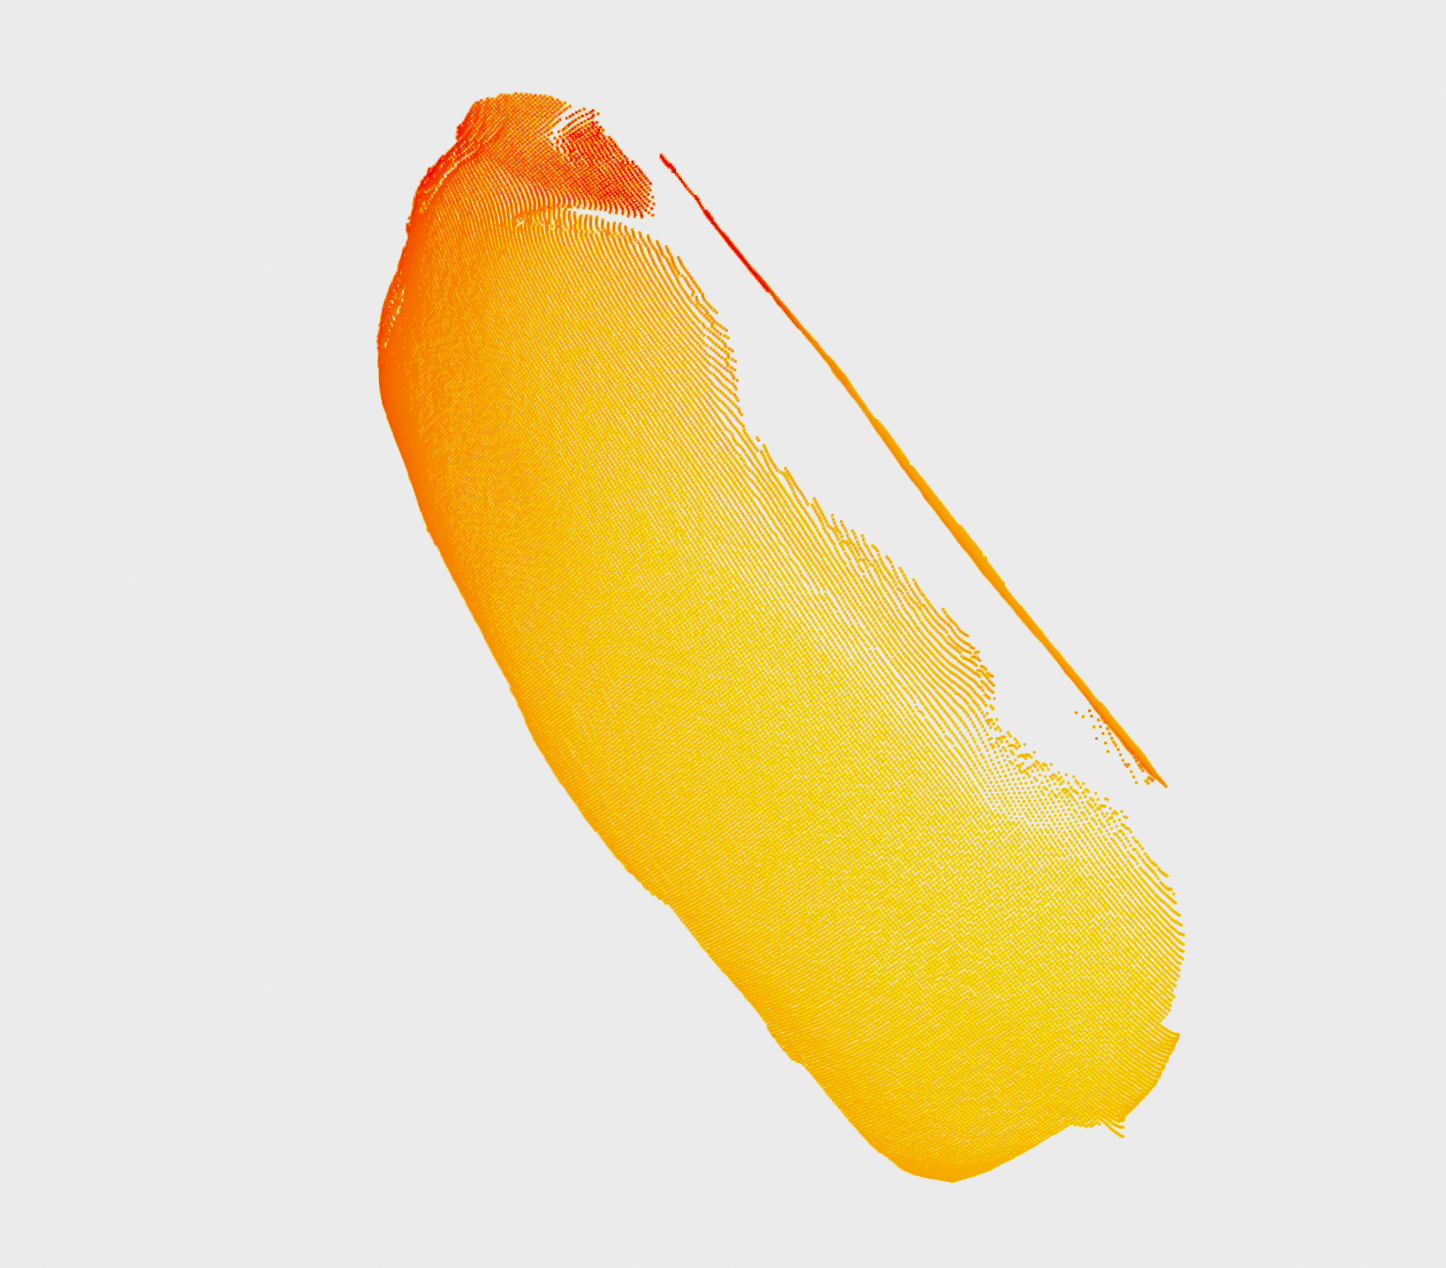
\includegraphics[width=0.3\textwidth]{05-TFG-template-latex/images/pcdmal.png}
\caption{Ejemplo de point cloud con pared}
\label{pcdmal}
\end{figure}

\begin{figure}[!]
\centering
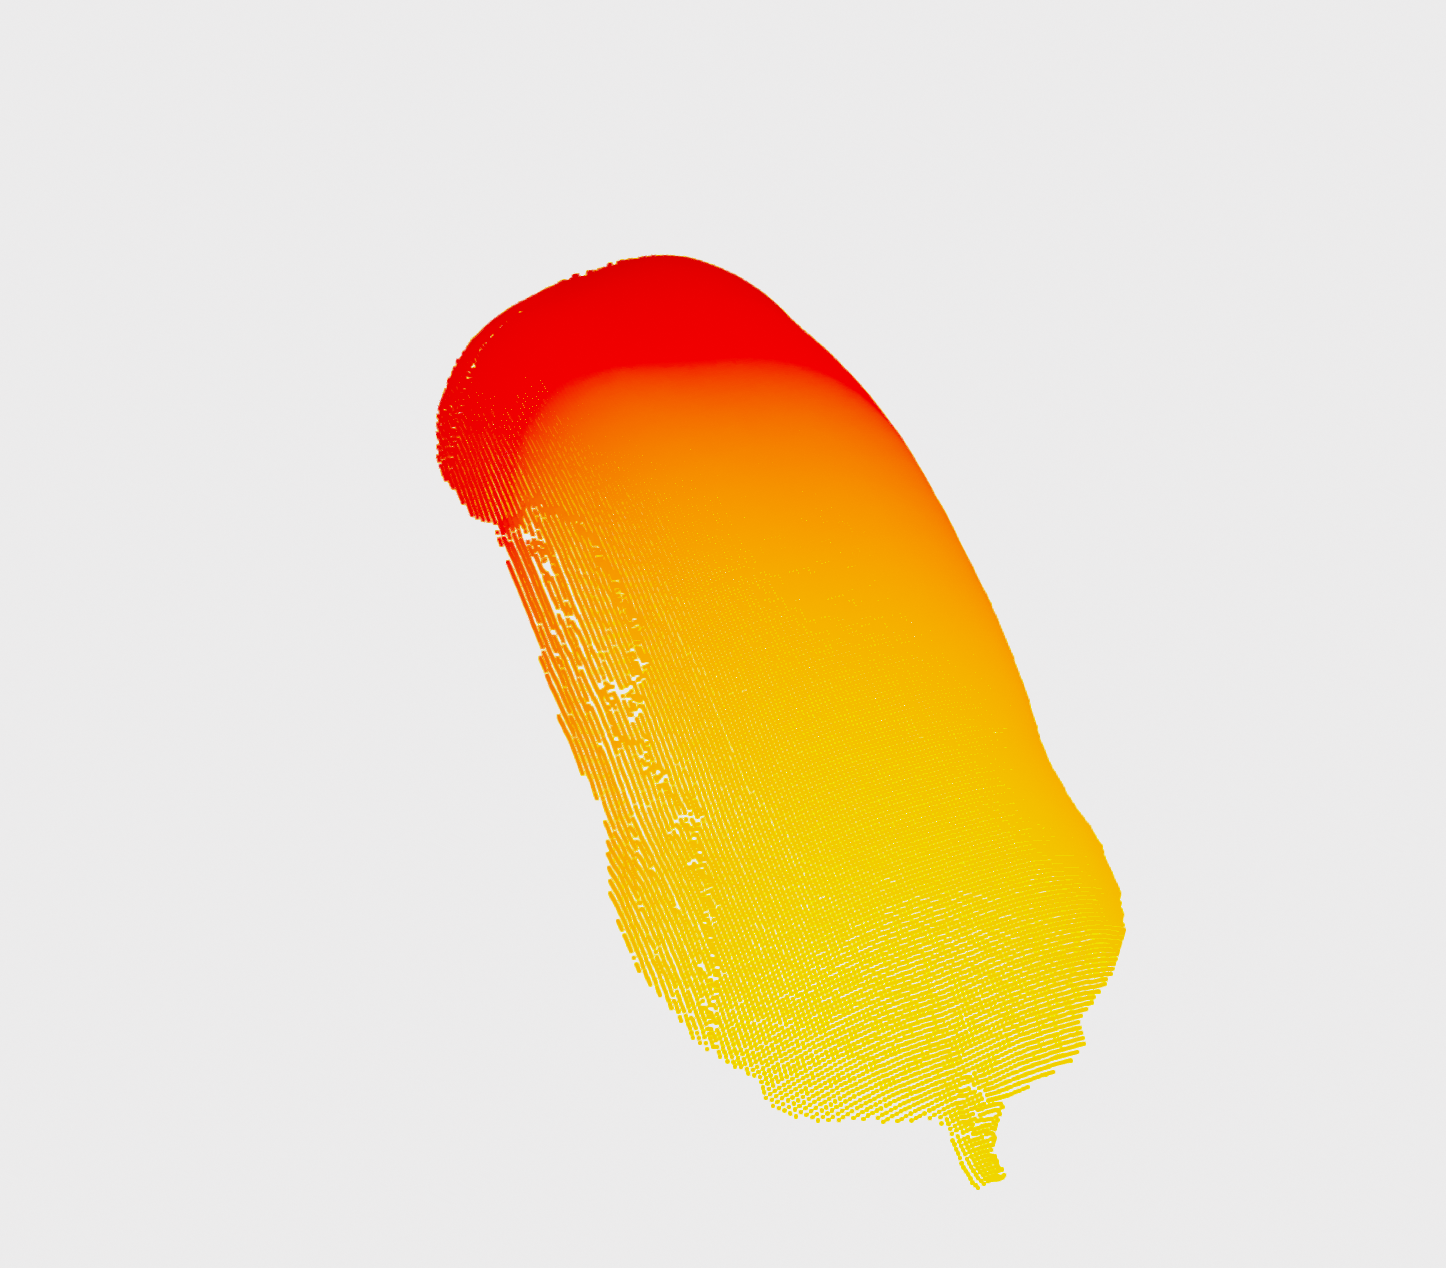
\includegraphics[width=0.3\textwidth]{05-TFG-template-latex/images/pcdbien.png}
\caption{Ejemplo de point cloud correcto}
\label{pcdbien}
\end{figure}

También se utilizó el groundtruth generado y un script de data augmentation para entrenar un modelo de segmentación semántica con ResNet50 \cite{resnet}, que debido a falta de potencia de cómputo no se ha podido realizar.

Desde el CVC usando las mascaras se han creado modelos de segmentación bastante eficaces como para substituir el método con Yolo, y como ya se ha comentado se está trabajando actualmente en una MobileNetV2 para intentar crear un nuevo método de segmentación propio, todo esto utilizando GoogleColab que presta potencia de cómputo de la que no disponemos.




Los accuracy de todos lo métodos se pueden consultar en la \textbf{TABLA \ref{acc}}.





Finalmente, se construye el modelo en 3D con open3D \cite{open3D} y se eliminan todos los puntos que se encuentran más abajo de un determinado lindar para así eliminar suelo, seguidamente se eliminan outlayers de manera estadística. Sin embargo, esta técnica debe mejorarse, en algunos casos no se detecta correctamente toda la superficie del cerdo, en otros casos se seleccionan puntos pertenecientes a la pared de la báscula como en la \textbf{Fig \ref{pcdmal}}. Otro aspecto a destacar serían las cabezas de los cerdos, algunos de ellos tienen la cabeza levantada y se segmenta su cabeza, otros la tienen agachada y no se segmenta correctamente. Un ejemplo nube de puntos sin errores sería la que se muestra en la \textbf{Fig \ref{pcdbien}}.








\begin{thebibliography}{5}

\bibitem{sistema}
    AHDB Pork \emph{"Pigs 2022 - Pig weighing systems"} [Online 30/9/2021]
    \url{https://www.youtube.com/watch?v=3CuLNYhFOjk}
    
\bibitem{camara}
    Basler \emph{"Basler blaze"} [Online 30/9/2021]
    \url{https://www.baslerweb.com/en/products/cameras/3d-cameras/basler-blaze/}

\bibitem{Area}
    K. Kollis, C.S. Phang, T.M. Banhazi and S.J. Searle \emph{"Weight estimation using image analysis and
    statistical modelling: A preliminary study"} [Online 30/9/2021]
    \url{https://www.researchgate.net/publication/236886740_Weight_Estimation_Using_Image_Analysis_and_Statistical_Modelling_A_Preliminary_Study}
\bibitem{3D}
    Dorota Anglart \emph{"Automatic estimation of body weight and body condition score in dairy cows using 3D imaging technique"} [Online 30/9/2021]
    \url{https://stud.epsilon.slu.se/6355/1/anglart_d_140114.pdf}
\bibitem{CNN}
    Jianlong Zhang, Yanrong Zhuang, Hengyi Ji, and Guanghui Teng \emph{"Pig Weight and Body Size Estimation Using a Multiple Output Regression Convolutional Neural Network: A Fast and Fully Automatic Method"} [Online 30/9/2021]
    \url{https://www.researchgate.net/publication/352102505_Pig_Weight_and_Body_Size_Estimation_Using_a_Multiple_Output_Regression_Convolutional_Neural_Network_A_Fast_and_Fully_Automatic_Method}
    
\bibitem{PLF}
    PLF Agritech \emph{"PLF Agritech"} [Online 30/9/2021]
    \url{http://plfag.com/technologies/}
    
\bibitem{fancom}
    Fancom \emph{"Fancom"} [Online 30/9/2021]
    \url{https://www.fancom.com}

\bibitem{fancomvideo}
    Fancom BV \emph{"eYeGrow - Weight monitor for finishers"} [Online 30/9/2021]
    \url{https://www.youtube.com/watch?v=CSuWWgY43PA}    

\bibitem{deteccion}
    Eric T. Psota, Mateusz Mittek, Lance Pérez and Ty B Schmidt \emph{"Multi-Pig Part Detection and Association with a Fully Convolutional Network"} [Online 30/9/2021]
    \url{https://www.researchgate.net/publication/352102505_Pig_Weight_and_Body_Size_Estimation_Using_a_Multiple_Output_Regression_Convolutional_Neural_Network_A_Fast_and_Fully_Automatic_Method}
    
\bibitem{GroStat}
    GroStat \emph{"GROWTH SENSOR"} [Online 30/9/2021]
    \url{http://grostat.com/growth_sensor.php#prettyPhoto}

\bibitem{H+L}
    H+L \emph{"optiSCAN"} [Online 30/9/2021]
    \url{https://hl-agrar.de/en_gb/optiscan/}

\bibitem{piggycheck}
    Agro Napló \emph{"Piggy Check – weigh pigs with your tablet PC"} [Online 30/9/2021]
    \url{https://www.agronaplo.hu/nagyvilag/piggy-check-weigh-pigs-with-your-tablet-pc}

\bibitem{japon}
    The Mainichi \emph{"Southwest Japan univ. develops smart glasses to visually estimate pigs' weight"} [Online 30/9/2021]
    \url{https://mainichi.jp/english/articles/20210601/p2a/00m/0na/007000c}

\bibitem{google}
    Glass \emph{"Glass"} [Online 30/9/2021]
    \url{https://www.google.com/glass/start/}

\bibitem{JIRA}
    Altassian \emph{"Jira"} [Online 30/9/2021]
    \url{https://www.atlassian.com/es/software/jira?}

\bibitem{degree}
    degree2act \emph{"degree2act"} [Online 30/9/2021]
    \url{https://www.degree2act.com/}
    
\bibitem{Otsu}
    LearnOpenCV \emph{"Otsu’s Thresholding with OpenCV"} [Online 10/11/2021]
    \url{https://learnopencv.com/Otsu-thresholding-with-opencv/}

\bibitem{hough}
    LearnOpenCV \emph{"Hough Transform with OpenCV (C++/Python)"} [Online 10/11/2021]
    \url{https://learnopencv.com/hough-transform-with-opencv-c-python/}

\bibitem{hasty}
    Hasty.ai \emph{"Hasty"} [Online 10/11/2021]
    \url{https://hasty.ai}

\bibitem{yolo}
    Yolov5 \emph{"ultralytics/yolov5"} [Online 10/11/2021]
    \url{https://github.com/ultralytics/yolov5}

\bibitem{Niblack}
    scikit-image \emph{"Niblack and Sauvola Thresholding"} [Online 10/11/2021]
    \url{http://www.open3d.org}

\bibitem{open3D}
    Open3D \emph{"Open3D"} [Online 10/11/2021]
    \url{http://www.open3d.org}

\bibitem{resnet}
    Kaiming He, Xiangyu Zhang, Shaoqing Ren and Jian Sun \emph{"Deep Residual Learning for Image Recognition"} [Online 10/11/2021]
    \url{https://arxiv.org/pdf/1512.03385.pdf}

\bibitem{mobilenet}
    Mark Sandler, Andrew Howard, Menglong Zhu, Andrey Zhmoginov and Liang-Chieh Chen \emph{"MobileNetV2: Inverted Residuals and Linear Bottlenecks"} [Online 10/11/2021]
    \url{https://arxiv.org/pdf/1801.04381.pdf}


\end{thebibliography}




\setcounter{section}{1}

\blfootnote{$\bullet$ E-mail de contacte: maldonadolorcamarc@gmail.com}
\blfootnote{$\bullet$ Menció realitzada: Computació}
\blfootnote{$\bullet$ Treball tutoritzat per: Coen Antens (CVC)}
\blfootnote{$\bullet$ Curs 2021/22}
\end{document}

